\documentclass[a4paper, 12pt]{article}

\usepackage[utf8]{inputenc}
\usepackage[T1, T2A]{fontenc}
\usepackage[english, russian]{babel}
\usepackage[top=2cm, bottom=2cm, left=2cm, right=2cm]{geometry}

\usepackage{pgfplots}
\pgfplotsset{compat=1.13}
\pgfplotsset{grid = major, grid style = {dashed}}

\usepackage{subcaption}
\usepackage{amsmath}

\usepackage{tabu}

% PGFPlots Table ========================================================
\usepackage{pgfplotstable}
\renewcommand{\arraystretch}{1.3}
% recommended:
\usepackage{booktabs}
\usepackage{colortbl}
% pgfplotstable settings
\pgfplotstableset{
    every head row/.style = {before row = \hline},
    after row = {[1mm] \hline},
    column type = {|c},
    every last column/.style={
        column type/.add={}{|},
    },   
}
\usepackage{threeparttable}
\renewcommand{\TPTminimum}{\linewidth}

% Paragraph indent
\usepackage{indentfirst}
\setlength{\parindent}{15mm}

%Change label separator
\usepackage{caption}
\captionsetup[table]{labelformat=simple, labelsep = endash, justification = raggedright, singlelinecheck = off, width = 0.75\textwidth}
\captionsetup[figure]{labelformat=simple, labelsep = endash, name = Рисунок}

\usepackage{../titlepage/TAYTitle}
\author{Овчаров Алексей}
\title{Исследование математической модели электромеханического объекта управления}
\labnumber{10}
\variant{3}

\begin{document}

\maketitle

\section{Задание}
\textbf{Цель работы} - изучение математических моделей и исследование характеристик электромеханического объекта управления, построенного на основе электродвигателя постоянного тока независимого возбуждения. \par
Необходимо по известной модели электромеханического объекта (ЭМО) построить схему и провести математическое моделирование при различных параметрах системы. Функциональная схема исследумого объекта представлена на рисунке 1.
\begin{figure} [h!]
    \centering
    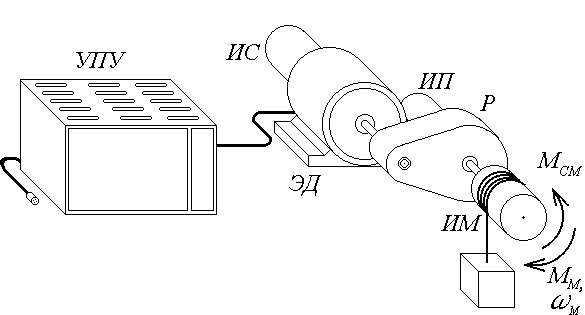
\includegraphics[width = 0.7\textwidth]{images/EMO.png}
    \caption{Функциональная схема ЭМО}
\end{figure} \par
Усилительно-преобразовательное устройство (УПУ) описывается следующим уравнением:
\begin{equation}
    T_y\dot{U_y} + U_y = K_yU
\end{equation} \par
УПУ подключается к электродвигателю (ЭД) - двигетлю постоянного тока (ДПТ), к которому пеодключен исполнительный механизм (ИМ) через редуктор (Р) с целью снизить момент на роторе двигателя. Описанную систему можно описать следующими уравнениями.
\begin{align}
    T_\text{я}\dot{I} + I & = K_\text{д}(U_y + K_e\omega_Mi_p) &
    K_\text{м} - \frac{M_\text{СМ}}{i_p} & = J_\Sigma\dot{\omega}_Mi &
    J_\Sigma & = J_\text{д} + J_p + \frac{J_M}{i_p^2}
\end{align} \par
Изменяя параметры $M_\text{СМ}$, $i_p$, $J_M$, $T_\text{я}$ и $T_y$ необходимо получить графики переходных процессов и сравнить их.

В таблице 1 представлены исходные данные для моделирования ДПТ.
\begin{table}[h!]
    \centering
    \begin{threeparttable}
        \caption{Исходные данные.}
        \begin{tabular}{|c|c|c|c|c|c|c|c|c|c|}
            \hline
            $U_\text{Н}$ & $n_0$ & $I_\text{Н}$ & $M_\text{Н}$ & $R$ & $U_\text{Я}$ & $J_\text{Д}$ & $T_\text{у}$ & $i_\text{р}$ & $J_\text{М}$\\
            В & об/мин & А & Н$\cdot$м & Ом & мс & кг$\cdot\text{м}^2$ & мс & &  кг$\cdot\text{м}^2$ \\ \hline
            36 & 4000 & 6.5 & 0.57 & 0.85 & 3 & $2.2\cdot10^{-4}$ & 6 & 40 & 0.15 \\
            \hline
        \end{tabular}
    \end{threeparttable}
\end{table}

\newpage
\section{Рассчет параметров моделирования}

По исходным данным можно рассчитать некоторые параметры моделирования.\par
\begin{align*}
    K_y & = \frac{U_\text{Н}}{U_m} = \frac{36}{10} = 3.6 & w_0 & = n_0\frac{\pi}{30} = 418.9 \\
    K_e & = \frac{U_\text{Н}}{w_0} = 0.086 & K_\text{Д} & = \frac{1}{R} = 1.2 \\
    K_\text{М} & = \frac{M_\text{Н}}{I_\text{Н}} =  0.088 & J_{\Sigma} & = 1.2J_\text{Д} + \frac{J_\text{М}}{i^2_p} = 3.6 \cdot 10^{-4}
\end{align*} \par
Коэффициенты передачи измерительных устройств можно найти предварительно промоделировав систему и выбрав максимальное время моделирования. В итоге получим следующие значения коэффициентов: 
\begin{align*}
    K_U & = \frac{\hat{U}_{ymax}}{U_\text{Н}} = \frac{10}{36} = 0.28  & K_I & = \frac{\hat{I}_{max}}{I_{max}} = \frac{10}{31.35} =  0.32\\
    K_\omega & = \frac{\hat{\omega}_{max}}{\omega_0} = \frac{10}{418.9} = 0.024 & K_\alpha & = \frac{\hat{\alpha}_{max}}{\alpha_{max}} = \frac{10}{5.54} = 1.8
\end{align*}

\newpage
\section{Вывод моделей ВСВ}
\subsection{Модель ВСВ полной модели ЭМО}
Для начала запишем все уравнения, описывающие работу ЭМО. Их возьмем из теории.

\begin{equation}
    \begin{cases}
        k_\text{м}I - M_c = J_\Sigma \dot{\omega} \\
        T_\text{я}\dot{I} + I = k_\text{д}U_y - k_\text{д}k_e\omega \\
        T_y\dot{U_y} + U_y = k_yU
    \end{cases} \Leftrightarrow
    \begin{cases}
        \dot{\omega} = \frac{k_\text{м}}{J_\Sigma}I - \frac{1}{J_\Sigma}M_c \\
        \dot{I} = - \frac{k_\text{д}k_e}{T_\text{я}}\omega - \frac{1}{T_\text{я}}I + \frac{k_\text{д}}{T_\text{я}}U_y \\
        \dot{U_y} = -\frac{1}{T_y}U_y + \frac{k_y}{T_y}U
    \end{cases}
\end{equation} \par
Теперь, приняв за вектор состояния $X = \begin{bmatrix} \alpha & \omega & I & U_y \end{bmatrix}^T$ и $\dot{\alpha} = \omega$, получим следующую модель вход состояние выход (ВСВ).

\begin{align}
    \begin{bmatrix}
        \dot{\alpha} \\
        \dot{\omega} \\
        \dot{I} \\
        \dot{U_y} 
    \end{bmatrix} & = 
    \begin{bmatrix}
        0 & 1 & 0 & 0 \\
        0 & 0 & \frac{k_\text{м}}{J_\Sigma} & 0 \\
        0 & -\frac{k_\text{д}k_e}{T_\text{я}} & - \frac{1}{T_\text{я}} & \frac{k_\text{д}}{T_\text{я}} \\
        0 & 0 & 0 & -\frac{1}{T_y}
    \end{bmatrix}
    \begin{bmatrix}
        \alpha \\
        \omega \\
        I \\
        U_y 
    \end{bmatrix} + 
    \begin{bmatrix}
        0 & 0 \\
        0 & - \frac{1}{J_\Sigma} \\
        0 & 0 \\
        \frac{k_y}{T_y} & 0
    \end{bmatrix}
    \begin{bmatrix}
        U(t) \\
        M_c(t)
    \end{bmatrix} \\
    \alpha & = 
    \begin{bmatrix}
        1 & 0 & 0 & 0
    \end{bmatrix}
    \begin{bmatrix}
        \alpha \\
        \omega \\
        I \\
        U_y 
    \end{bmatrix}
\end{align}

\subsection{Модель ВСВ упрощенной модели ЭМО}
Приравнивая в выражениях (3) $T_\text{я}$ и $T_y$ к 0. Получим следующие выражения:

\begin{equation}
    \begin{cases}
    \dot{\alpha} = \omega \\
    \dot{\omega} = -\frac{k_\text{м}k_\text{д}k_e}{J_\Sigma}\omega + \frac{k_\text{м}k_\text{д}k_y}{J_\Sigma}U - \frac{1}{J_\Sigma}M_c
    \end{cases}
\end{equation}

И соответственно модель ВСВ: 
\begin{align}
    \begin{bmatrix}
        \dot{\alpha} \\
        \dot{\omega} \\
    \end{bmatrix} & = 
    \begin{bmatrix}
        0 & 1 \\
        0 & -\frac{k_\text{м}k_\text{д}k_e}{J_\Sigma} \\
    \end{bmatrix}
    \begin{bmatrix}
        \alpha \\
        \omega \\
    \end{bmatrix} + 
    \begin{bmatrix}
        0 & 0 \\
        \frac{k_\text{м}k_\text{д}k_y}{J_\Sigma} & -\frac{1}{J_\Sigma} \\
    \end{bmatrix}
    \begin{bmatrix}
        U(t) \\
        M_c(t)
    \end{bmatrix} \\
    \alpha & = 
    \begin{bmatrix}
        1 & 0 
    \end{bmatrix}
    \begin{bmatrix}
        \alpha \\
        \omega \\
    \end{bmatrix}
\end{align}

\newpage
\section{Моделирование полной модели ЭМО}

На рисунке 1 представлна полная модель ДПТ.
\begin{figure}[h!]
    \centering
    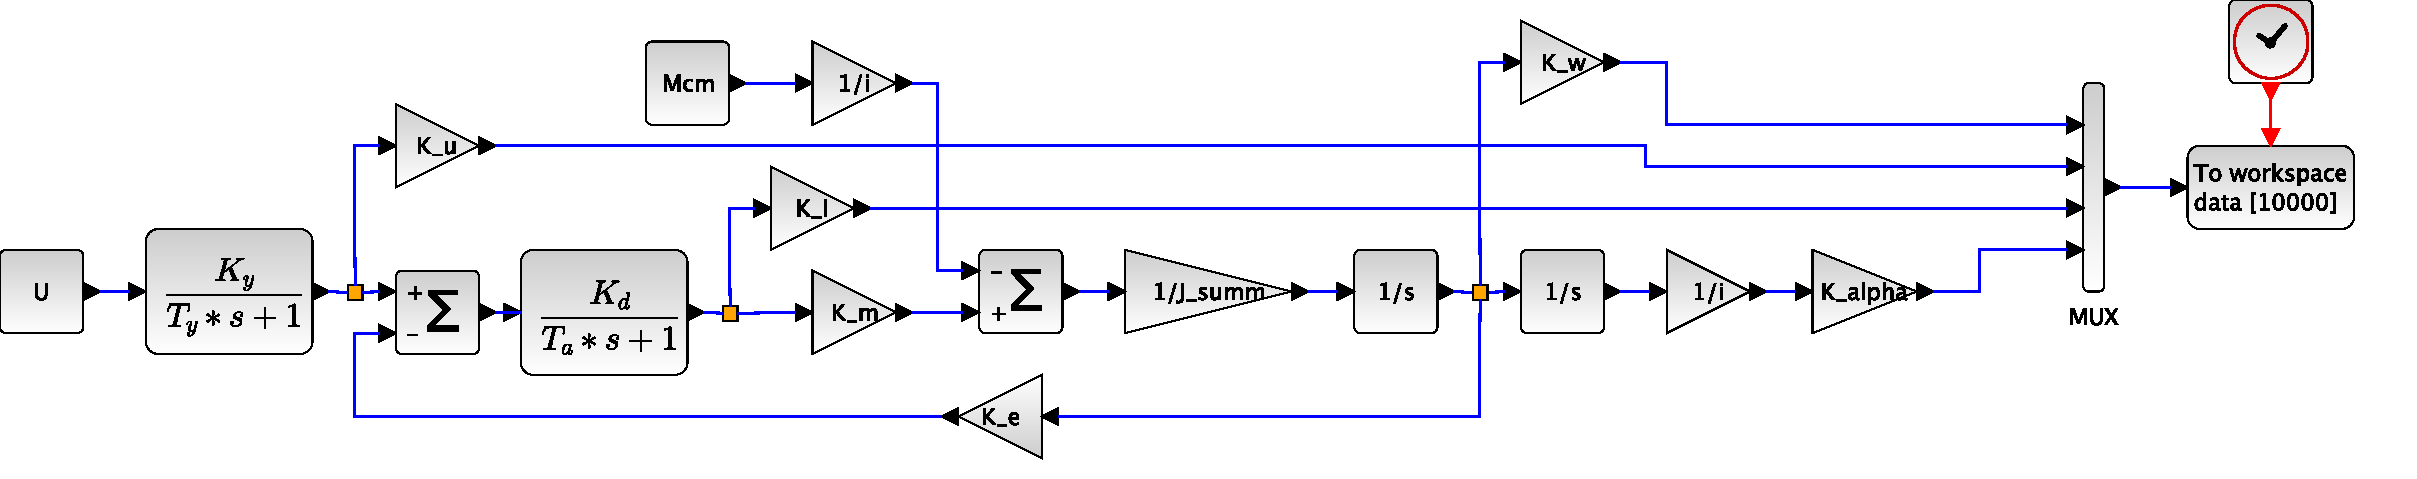
\includegraphics[width = \textwidth]{images/FullModel/full-model.pdf}
    \caption{Полная модель ЭМО}
\end{figure}

После построения модели и определения параметров моделирования можно получить графики и подсчитать соответственно время переходного процесса $t_\text{п}$, установившиеся угловую скорость $\omega_y$ и ток $I_y$.

\begin{align*}
    t_\text{п} & = 0.036 & \omega_y & = 5 & I_y & = 0.0031 \\
\end{align*}

Ниже предсавлены графки переходных процессов двигателя при $T_y = 6\cdot10^{-3}$ c и $T_\text{Я} = 3\cdot10^{-3}$ c.

\begin{figure}[h!]
    \centering
    \begin{tikzpicture}
        \begin{axis} [
            width = 0.7\textwidth,
            height = 7cm,
            xlabel = {$t$, c},
            ylabel = {$\omega$, 1/c},
            grid = major,
            grid style = {dashed},
            xmin = 0, xmax = 0.3,
        ]
            \addplot[blue, mark = none, thick, smooth, solid] table [x = t, y = w] {data/FullModel/TransPlot.dat};
            \addplot[blue, mark = none, thick, smooth, dashed] table [x = t, y = I] {data/FullModel/TransPlot.dat};
            \addplot[blue, mark = none, thick, smooth, dotted] table [x = t, y = alpha] {data/FullModel/TransPlot.dat};
            \addplot[blue, mark = none, thick, smooth, dashdotted] table [x = t, y = U] {data/FullModel/TransPlot.dat};
            \legend{$\omega$, $I$, $\alpha_M$,$U$};
        \end{axis}
    \end{tikzpicture}
    \caption{Переходные процессы в ДПТ}
\end{figure}

\newpage
Ниже предсавлены графки переходных процессов двигателя при $T_y = 6\cdot10^{-4}$ c и $T_\text{Я} = 3\cdot10^{-4}$ c.

\begin{figure}[h!]
    \centering
    \begin{tikzpicture}
        \begin{axis} [
            width = 0.7\textwidth,
            height = 7cm,
            xlabel = {$t$, c},
            ylabel = {$\omega$, 1/c},
            grid = major,
            grid style = {dashed},
            xmin = 0, xmax = 0.3,
        ]
            \addplot[blue, mark = none, thick, smooth, solid] table [x = t, y = w] {data/FullModel/TransPlotSwitchedTime.dat};
            \addplot[blue, mark = none, thick, smooth, dashed] table [x = t, y = I] {data/FullModel/TransPlotSwitchedTime.dat};
            \addplot[blue, mark = none, thick, smooth, dotted] table [x = t, y = alpha] {data/FullModel/TransPlotSwitchedTime.dat};
            \addplot[blue, mark = none, thick, smooth, dashdotted] table [x = t, y = U] {data/FullModel/TransPlotSwitchedTime.dat};
            \legend{$\omega$, $I$, $\alpha$,$U$};
        \end{axis}
    \end{tikzpicture}
    \caption{Переходные процессы в ДПТ при меньших значениях постоянных времени}
\end{figure}

Также по графику переходного процесса можно определить время переходного процесса и установившиеся значения тока и угловой скорости.
\begin{align*}
    t_\text{п} & = 0.029 & \omega_y & = 5 & I_y & = 0.004 \\
\end{align*}

\newpage
\section{Исследование влияния момента сопротивленя $M_\text{СМ}$}
На рисунке 5 представлены переходные процессы ДПТ при различных значениях нагрузочного момента $M_\text{СМ}$.


\begin{figure}[h!]
    \begin{subfigure}{0.5\textwidth}
        \centering
        \begin{tikzpicture} 
            \begin{axis} [
                width = 0.9\textwidth,
                ylabel = {$\omega$, 1/c},
                xlabel = {$t$, c},
                legend pos=south east,
                grid = major,
                grid style = {dashed},
                xmin = 0, xmax = 0.3,
                extra y ticks={5, 4.61, 4.23, 3.85, 3.46},
                extra y tick style={grid style={black, thick, dashed}},
                ytick = {0, 2},
            ]
                \addplot[blue, mark = none, thick, smooth, solid] table [x = t, y = w1] {data/FullModel/Moment-w.dat};
                \addplot[blue, mark = none, thick, smooth, dashed] table [x = t, y = w2] {data/FullModel/Moment-w.dat};
                \addplot[blue, mark = none, thick, smooth, dotted] table [x = t, y = w3] {data/FullModel/Moment-w.dat};
                \addplot[blue, mark = none, thick, smooth, densely dashed] table [x = t, y = w4] {data/FullModel/Moment-w.dat};
                \addplot[blue, mark = none, thick, smooth, dashdotted] table [x = t, y = w5] {data/FullModel/Moment-w.dat};
                \legend{$M_{cm} = 0$, $M_{cm} = 5.7$, $M_{cm} = 11.4$, $M_{cm} = 17.1$, $M_{cm} = 22.8$};
            \end{axis}
        \end{tikzpicture}
    \end{subfigure}
    \begin{subfigure}{0.5\textwidth}
        \centering
        \begin{tikzpicture} 
            \begin{axis} [
                width = 0.9\textwidth,
                ylabel = {$I$, A},
                xlabel = {$t$, c},
                legend pos=north east,
                grid = major,
                grid style = {dashed},
                xmin = 0, xmax = 0.3,
                extra y ticks={0, 0.52, 1.04, 1.56, 2.08},
                extra y tick style={grid style={black, thick, dashed}},
                ytick = {4, 6},
            ]
                \addplot[blue, mark = none, thick, smooth, solid] table [x = t, y = I1] {data/FullModel/Moment-I.dat};
                \addplot[blue, mark = none, thick, smooth, dashed] table [x = t, y = I2] {data/FullModel/Moment-I.dat};
                \addplot[blue, mark = none, thick, smooth, dotted] table [x = t, y = I3] {data/FullModel/Moment-I.dat};
                \addplot[blue, mark = none, thick, smooth, densely dashed] table [x = t, y = I4] {data/FullModel/Moment-I.dat};
                \addplot[blue, mark = none, thick, smooth, dashdotted] table [x = t, y = I5] {data/FullModel/Moment-I.dat};
                \legend{$M_{cm} = 0$, $M_{cm} = 5.7$, $M_{cm} = 11.4$, $M_{cm} = 17.1$, $M_{cm} = 22.8$};
            \end{axis}
        \end{tikzpicture}
    \end{subfigure}
    \vspace{0.5cm}

    \begin{subfigure}{0.5\textwidth}
        \centering
        \begin{tikzpicture} 
            \begin{axis} [
                width = 0.9\textwidth,
                ylabel = {$\alpha_M$, \text{градусы}},
                xlabel = {$t$, c},
                legend pos=north west,
                grid = major,
                grid style = {dashed},
                xmin = 0, xmax = 0.3,
            ]
                \addplot[blue, mark = none, thick, smooth, solid] table [x = t, y = alpha1] {data/FullModel/Moment-alpha.dat};
                \addplot[blue, mark = none, thick, smooth, dashed] table [x = t, y = alpha2] {data/FullModel/Moment-alpha.dat};
                \addplot[blue, mark = none, thick, smooth, dotted] table [x = t, y = alpha3] {data/FullModel/Moment-alpha.dat};
                \addplot[blue, mark = none, thick, smooth, densely dashed] table [x = t, y = alpha4] {data/FullModel/Moment-alpha.dat};
                \addplot[blue, mark = none, thick, smooth, dashdotted] table [x = t, y = alpha5] {data/FullModel/Moment-alpha.dat};
                \legend{$M_{cm} = 0$, $M_{cm} = 5.7$, $M_{cm} = 11.4$, $M_{cm} = 17.1$, $M_{cm} = 22.8$};
            \end{axis}
        \end{tikzpicture}
    \end{subfigure}
    \begin{subfigure}{0.5\textwidth}
        \centering
        \begin{tikzpicture} 
            \begin{axis} [
                width = 0.9\textwidth,
                ylabel = {$U$, B},
                xlabel = {$t$, c},
                legend pos=south east,
                grid = major,
                grid style = {dashed},
                xmin = 0, xmax = 0.3,
            ]

                \addplot[blue, mark = none, thick, smooth, solid] table [x = t, y = U1] {data/FullModel/Moment-U.dat};
            \end{axis}
        \end{tikzpicture}
    \end{subfigure}
    \caption{Графики прехеходных процессов при различных $M_\text{СМ}$}
\end{figure}

В ходе эксперимента, изменяя нагрузочный момент, мы получили различные значения времени переходного процесса и установившиеся значения тока и угловой скорости, которые представлены в таблице ниже.

\begin{table}[h!]
    \centering
    \begin{threeparttable}
        \caption{Данные о перехоных процессах при изменении момента нагрузки}
        \pgfplotstabletypeset[
            columns/t_p/.style = {column name = {$t_\text{п}$}},
            columns/w/.style = {column name = {$\omega_y$}},
            columns/I/.style = {column name = {$I_y$}},
            columns/M/.style = {column name = {$M_\text{СМ}$}},
        ]{data/FullModel/Moment.dat}
    \end{threeparttable}
\end{table}

\newpage
\section{Исследование влеяния момента инерции нагрузки $J_\text{М}$}
На рисунке 6 представлены графики переходных процессов при различных значениях момента инерции нагрузки $J_\text{М}$.

\begin{figure}[h!]
    \begin{subfigure}{0.5\textwidth}
        \centering
        \begin{tikzpicture} 
            \begin{axis} [
                width = 0.9\textwidth,
                ylabel = {$\omega$, 1/c},
                xlabel = {$t$, c},
                legend pos=south east,
                grid = major,
                grid style = {dashed},
                xmin = 0, xmax = 0.3,
            ]
                \addplot[blue, mark = none, thick, smooth, solid] table [x = t, y = w1] {data/FullModel/InertiaMoment-w.dat};
                \addplot[blue, mark = none, thick, smooth, dashed] table [x = t, y = w2] {data/FullModel/InertiaMoment-w.dat};
                \addplot[blue, mark = none, thick, smooth, dotted] table [x = t, y = w3] {data/FullModel/InertiaMoment-w.dat};
                \addplot[blue, mark = none, thick, smooth, densely dashed] table [x = t, y = w4] {data/FullModel/InertiaMoment-w.dat};
                \addplot[blue, mark = none, thick, smooth, dashdotted] table [x = t, y = w5] {data/FullModel/InertiaMoment-w.dat};
                \legend{$J_{M} = 0.075$, $J_{M} = 0.11$, $J_{M} = 0.15$, $J_{M} = 0.19$, $J_{M} = 0.23$};
            \end{axis}
        \end{tikzpicture}
    \end{subfigure}
    \begin{subfigure}{0.5\textwidth}
        \centering
        \begin{tikzpicture} 
            \begin{axis} [
                width = 0.9\textwidth,
                ylabel = {$I$, A},
                xlabel = {$t$, c},
                legend pos=north east,
                grid = major,
                grid style = {dashed},
                xmin = 0, xmax = 0.3,
            ]
                \addplot[blue, mark = none, thick, smooth, solid] table [x = t, y = I1] {data/FullModel/InertiaMoment-I.dat};
                \addplot[blue, mark = none, thick, smooth, dashed] table [x = t, y = I2] {data/FullModel/InertiaMoment-I.dat};
                \addplot[blue, mark = none, thick, smooth, dotted] table [x = t, y = I3] {data/FullModel/InertiaMoment-I.dat};
                \addplot[blue, mark = none, thick, smooth, densely dashed] table [x = t, y = I4] {data/FullModel/InertiaMoment-I.dat};
                \addplot[blue, mark = none, thick, smooth, dashdotted] table [x = t, y = I5] {data/FullModel/InertiaMoment-I.dat};
                \legend{$J_{M} = 0.075$, $J_{M} = 0.11$, $J_{M} = 0.15$, $J_{M} = 0.19$, $J_{M} = 0.23$};
            \end{axis}
        \end{tikzpicture}
    \end{subfigure}
    \vspace{0.5cm}

    \begin{subfigure}{0.5\textwidth}
        \centering
        \begin{tikzpicture} 
            \begin{axis} [
                width = 0.9\textwidth,
                ylabel = {$\alpha_M$, \text{градусы}},
                xlabel = {$t$, c},
                legend pos=north west,
                grid = major,
                grid style = {dashed},
                xmin = 0, xmax = 0.3,
            ]
                \addplot[blue, mark = none, thick, smooth, solid] table [x = t, y = alpha1] {data/FullModel/InertiaMoment-alpha.dat};
                \addplot[blue, mark = none, thick, smooth, dashed] table [x = t, y = alpha2] {data/FullModel/InertiaMoment-alpha.dat};
                \addplot[blue, mark = none, thick, smooth, dotted] table [x = t, y = alpha3] {data/FullModel/InertiaMoment-alpha.dat};
                \addplot[blue, mark = none, thick, smooth, densely dashed] table [x = t, y = alpha4] {data/FullModel/InertiaMoment-alpha.dat};
                \addplot[blue, mark = none, thick, smooth, dashdotted] table [x = t, y = alpha5] {data/FullModel/InertiaMoment-alpha.dat};
                \legend{$J_{M} = 0.075$, $J_{M} = 0.11$, $J_{M} = 0.15$, $J_{M} = 0.19$, $J_{M} = 0.23$};
            \end{axis}
        \end{tikzpicture}
    \end{subfigure}
    \begin{subfigure}{0.5\textwidth}
        \centering
        \begin{tikzpicture} 
            \begin{axis} [
                width = 0.9\textwidth,
                ylabel = {$U$, B},
                xlabel = {$t$, c},
                legend pos=south east,
                grid = major,
                grid style = {dashed},
                xmin = 0, xmax = 0.3,
            ]
                \addplot[blue, mark = none, thick, smooth, solid] table [x = t, y = U1] {data/FullModel/InertiaMoment-U.dat};
            \end{axis}
        \end{tikzpicture}
    \end{subfigure}
    \caption{Графики прехеходных процессов при различных $J_\text{М}$}
\end{figure}

В ходе эксперимента, изменяя момент инерции нагрузки, мы получили различные значения времени переходного процесса и установившиеся значения тока и угловой скорости, которые представлены в таблице ниже.

\begin{table}[h!]
    \centering
    \begin{threeparttable}
        \caption{Данные о перехоных процессах при изменении момента инерции нагрузки.}
        \pgfplotstabletypeset[
            columns/t_p/.style = {column name = {$t_\text{п}$}},
            columns/w/.style = {column name = {$\omega_y$}},
            columns/I/.style = {column name = {$I_y$}},
            columns/J/.style = {column name = {$J_\text{М}$}},
        ]{data/FullModel/InertiaMoment.dat}
    \end{threeparttable}
\end{table}

\newpage
\section{Исследование влияния передаточного отношения $i_p$ редукотора}
На рисунке 7 представлены графики преходных процессов при различных значениях передаточного отношения и нулевом моменте нагрузки $M_\text{СМ} = 0$.

\begin{figure}[h!]
    \begin{subfigure}{0.5\textwidth}
        \centering
        \begin{tikzpicture} 
            \begin{axis} [
                width = 0.9\textwidth,
                ylabel = {$\omega$, 1/c},
                xlabel = {$t$, c},
                legend pos=south east,
                grid = major,
                grid style = {dashed},
                xmin = 0, xmax = 0.9,
                extra y ticks={5},
                extra tick style={grid=major},
            ]
                \addplot[blue, mark = none, thick, smooth, solid] table [x = t, y = w1] {data/FullModel/GearRatio-w.dat};
                \addplot[blue, mark = none, thick, smooth, dashed] table [x = t, y = w2] {data/FullModel/GearRatio-w.dat};
                \addplot[blue, mark = none, thick, smooth, dotted] table [x = t, y = w3] {data/FullModel/GearRatio-w.dat};
                \addplot[blue, mark = none, thick, smooth, densely dashed] table [x = t, y = w4] {data/FullModel/GearRatio-w.dat};
                \addplot[blue, mark = none, thick, smooth, dashdotted] table [x = t, y = w5] {data/FullModel/GearRatio-w.dat};
                \legend{$i_{p} = 10$, $i_{p} = 25$, $i_{p} = 40$, $i_{p} = 55$, $i_{p} = 70$};
            \end{axis}
        \end{tikzpicture}
    \end{subfigure}
    \begin{subfigure}{0.5\textwidth}
        \centering
        \begin{tikzpicture} 
            \begin{axis} [
                width = 0.9\textwidth,
                ylabel = {$I$, A},
                xlabel = {$t$, c},
                legend pos=north east,
                grid = major,
                grid style = {dashed},
                xmin = 0, xmax = 0.9,
            ]
                \addplot[blue, mark = none, thick, smooth, solid] table [x = t, y = I1] {data/FullModel/GearRatio-I.dat};
                \addplot[blue, mark = none, thick, smooth, dashed] table [x = t, y = I2] {data/FullModel/GearRatio-I.dat};
                \addplot[blue, mark = none, thick, smooth, dotted] table [x = t, y = I3] {data/FullModel/GearRatio-I.dat};
                \addplot[blue, mark = none, thick, smooth, densely dashed] table [x = t, y = I4] {data/FullModel/GearRatio-I.dat};
                \addplot[blue, mark = none, thick, smooth, dashdotted] table [x = t, y = I5] {data/FullModel/GearRatio-I.dat};
                \legend{$i_{p} = 10$, $i_{p} = 25$, $i_{p} = 40$, $i_{p} = 55$, $i_{p} = 70$};
            \end{axis}
        \end{tikzpicture}
    \end{subfigure}
    \vspace{0.5cm}

    \begin{subfigure}{0.5\textwidth}
        \centering
        \begin{tikzpicture} 
            \begin{axis} [
                width = 0.9\textwidth,
                ylabel = {$\alpha_M$, \text{градусы}},
                xlabel = {$t$, c},
                legend pos=north west,
                grid = major,
                grid style = {dashed},
                xmin = 0, xmax = 0.9,
            ]
                \addplot[blue, mark = none, thick, smooth, solid] table [x = t, y = alpha1] {data/FullModel/GearRatio-alpha.dat};
                \addplot[blue, mark = none, thick, smooth, dashed] table [x = t, y = alpha2] {data/FullModel/GearRatio-alpha.dat};
                \addplot[blue, mark = none, thick, smooth, dotted] table [x = t, y = alpha3] {data/FullModel/GearRatio-alpha.dat};
                \addplot[blue, mark = none, thick, smooth, densely dashed] table [x = t, y = alpha4] {data/FullModel/GearRatio-alpha.dat};
                \addplot[blue, mark = none, thick, smooth, dashdotted] table [x = t, y = alpha5] {data/FullModel/GearRatio-alpha.dat};
                \legend{$i_{p} = 10$, $i_{p} = 25$, $i_{p} = 40$, $i_{p} = 55$, $i_{p} = 70$};
            \end{axis}
        \end{tikzpicture}
    \end{subfigure}
    \begin{subfigure}{0.5\textwidth}
        \centering
        \begin{tikzpicture} 
            \begin{axis} [
                width = 0.9\textwidth,
                ylabel = {$U$, B},
                xlabel = {$t$, c},
                legend pos=south east,
                grid = major,
                grid style = {dashed},
                xmin = 0, xmax = 0.9,
            ]
                \addplot[blue, mark = none, thick, smooth, solid] table [x = t, y = U1] {data/FullModel/GearRatio-U.dat};
            \end{axis}
        \end{tikzpicture}
    \end{subfigure}
    \caption{Графики прехеходных процессов при различных $i_p$ и $M_\text{СМ} = 0$}
\end{figure}

В ходе эксперимента, изменяя момент передаточное отношение редукторы, мы получили различные значения времени переходного процесса и установившиеся значения тока и угловой скорости, которые представлены в таблице ниже.

\begin{table}[h!]
    \centering
    \begin{threeparttable}
        \caption{Данные о перехоных процессах при изменении передаточного числа редуктора.}
        \pgfplotstabletypeset[
            columns/t_p/.style = {column name = {$t_\text{п}$}},
            columns/w/.style = {column name = {$\omega_y$}},
            columns/I/.style = {column name = {$I_y$}},
            columns/t/.style = {column name = {$i_{p}$}},
        ]{data/FullModel/GearRatio.dat}
    \end{threeparttable}
\end{table}

На рисунке 8 представлены графики преходных процессов при различных значениях передаточного отношения и не нулевом моменте нагрузки $M_\text{СМ} = M_\text{Н}i_p/2$, при $i_p = 40$.

\begin{figure}[h!]
    \begin{subfigure}{0.5\textwidth}
        \centering
        \begin{tikzpicture} 
            \begin{axis} [
                width = 0.9\textwidth,
                ylabel = {$\omega$, 1/c},
                xlabel = {$t$, c},
                legend pos=south east,
                grid = major,
                grid style = {dashed},
                xmin = 0, xmax = 0.9,
                extra y ticks={4.56, 4.44, 4.23, 3.77, 1.93},
                extra y tick labels={4.56, , 4.23, 3.77, 1.93},
                extra y tick style={grid style={black, thick, dashed}},
                ytick = {0, 1, 3},
                after end axis/.code={
                    \node  at (axis cs:0.9,4.16) [anchor=south west, align=left] {4.44};
                }
            ]
                \addplot[blue, mark = none, thick, smooth, solid] table [x = t, y = w1] {data/FullModel/GearRatioWithMoment-w.dat};
                \addplot[blue, mark = none, thick, smooth, dashed] table [x = t, y = w2] {data/FullModel/GearRatioWithMoment-w.dat};
                \addplot[blue, mark = none, thick, smooth, dotted] table [x = t, y = w3] {data/FullModel/GearRatioWithMoment-w.dat};
                \addplot[blue, mark = none, thick, smooth, densely dashed] table [x = t, y = w4] {data/FullModel/GearRatioWithMoment-w.dat};
                \addplot[blue, mark = none, thick, smooth, dashdotted] table [x = t, y = w5] {data/FullModel/GearRatioWithMoment-w.dat};
                \legend{$i_{p} = 10$, $i_{p} = 25$, $i_{p} = 40$, $i_{p} = 55$, $i_{p} = 70$};
            \end{axis}
        \end{tikzpicture}
    \end{subfigure}
    \begin{subfigure}{0.5\textwidth}
        \centering
        \begin{tikzpicture} 
            \begin{axis} [
                width = 0.9\textwidth,
                ylabel = {$I$, A},
                xlabel = {$t$, c},
                legend pos=north east,
                grid = major,
                grid style = {dashed},
                xmin = 0, xmax = 0.9,
                extra y ticks={4.15, 1.66, 1.04, 0.75, 0.59},
                extra y tick labels={4.15, 1.66, 1.04, , 0.59},
                extra y tick style={grid style={black, thick, dashed}},
                ytick = {0, 6},
                after end axis/.code={
                    \node  at (axis cs:0.9,0.4) [anchor=south west, align=left] {0.75};
                }
            ]
                \addplot[blue, mark = none, thick, smooth, solid] table [x = t, y = I1] {data/FullModel/GearRatioWithMoment-I.dat};
                \addplot[blue, mark = none, thick, smooth, dashed] table [x = t, y = I2] {data/FullModel/GearRatioWithMoment-I.dat};
                \addplot[blue, mark = none, thick, smooth, dotted] table [x = t, y = I3] {data/FullModel/GearRatioWithMoment-I.dat};
                \addplot[blue, mark = none, thick, smooth, densely dashed] table [x = t, y = I4] {data/FullModel/GearRatioWithMoment-I.dat};
                \addplot[blue, mark = none, thick, smooth, dashdotted] table [x = t, y = I5] {data/FullModel/GearRatioWithMoment-I.dat};
                \legend{$i_{p} = 10$, $i_{p} = 25$, $i_{p} = 40$, $i_{p} = 55$, $i_{p} = 70$};
            \end{axis}
        \end{tikzpicture}
    \end{subfigure}
    \vspace{0.5cm}

    \begin{subfigure}{0.5\textwidth}
        \centering
        \begin{tikzpicture} 
            \begin{axis} [
                width = 0.9\textwidth,
                ylabel = {$\alpha_M$, \text{градусы}},
                xlabel = {$t$, c},
                legend pos=north west,
                grid = major,
                grid style = {dashed},
                xmin = 0, xmax = 0.9,
            ]
                \addplot[blue, mark = none, thick, smooth, solid] table [x = t, y = alpha1] {data/FullModel/GearRatioWithMoment-alpha.dat};
                \addplot[blue, mark = none, thick, smooth, dashed] table [x = t, y = alpha2] {data/FullModel/GearRatioWithMoment-alpha.dat};
                \addplot[blue, mark = none, thick, smooth, dotted] table [x = t, y = alpha3] {data/FullModel/GearRatioWithMoment-alpha.dat};
                \addplot[blue, mark = none, thick, smooth, densely dashed] table [x = t, y = alpha4] {data/FullModel/GearRatioWithMoment-alpha.dat};
                \addplot[blue, mark = none, thick, smooth, dashdotted] table [x = t, y = alpha5] {data/FullModel/GearRatioWithMoment-alpha.dat};
                \legend{$i_{p} = 10$, $i_{p} = 25$, $i_{p} = 40$, $i_{p} = 55$, $i_{p} = 70$};
            \end{axis}
        \end{tikzpicture}
    \end{subfigure}
    \begin{subfigure}{0.5\textwidth}
        \centering
        \begin{tikzpicture} 
            \begin{axis} [
                width = 0.9\textwidth,
                ylabel = {$U$, B},
                xlabel = {$t$, c},
                legend pos=south east,
                grid = major,
                grid style = {dashed},
                xmin = 0, xmax = 0.9,
            ]
                \addplot[blue, mark = none, thick, smooth, solid] table [x = t, y = U1] {data/FullModel/GearRatioWithMoment-U.dat};
            \end{axis}
        \end{tikzpicture}
    \end{subfigure}
    \caption{Графики прехеходных процессов при различных $i_p$ и $M_\text{СМ} = M_\text{Н}i_p/2$}
\end{figure}

В ходе эксперимента, изменяя момент передаточное отношение редукторы, мы получили различные значения времени переходного процесса и установившиеся значения тока и угловой скорости, которые представлены в таблице ниже.

\begin{table}[h!]
    \centering
    \begin{threeparttable}
        \caption{Данные о перехоных процессах при изменении передаточного числа редуктора.}
        \pgfplotstabletypeset[
            columns/t_p/.style = {column name = {$t_\text{п}$}},
            columns/w/.style = {column name = {$\omega_y$}},
            columns/I/.style = {column name = {$I_y$}},
            columns/t/.style = {column name = {$i_{p}$}},
        ]{data/FullModel/GearRatioWithMoment.dat}
        \end{threeparttable}
\end{table}

\newpage
\section{Сравнение плоной и упрощенной модели ЭМО}

Моделируемая система изображена на рисунке ниже.

\begin{figure}[h!]
    \centering
    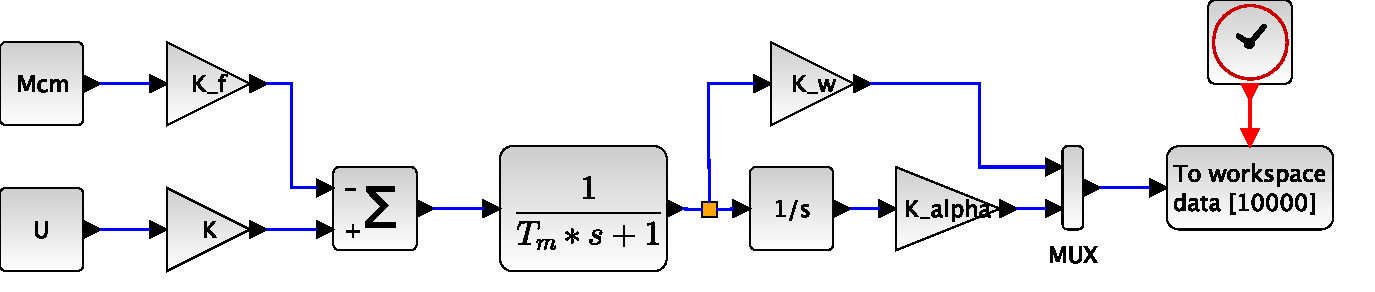
\includegraphics[width = 0.7\textwidth]{images/EasyModel/easy-model.pdf}
    \caption{Упрощенная модель ЭМО}
\end{figure}

\subsection{Сравнение моделей при при $T_\text{я} = 3\cdot10^{-3}$ и $T_\text{у} = 3\cdot10^{-3}$}
Ниже указаны характеристики переходного процесса упрощенной модели ЭМО. А также представлен график, в котором сравниваются полная и упрощенная модель.
\begin{align*}
    t_\text{п} & = 0.028 & \omega_y & = 5 \\
\end{align*}

\begin{figure}[h!]
    \centering
    \begin{tikzpicture}
        \begin{axis} [
            width = 0.85\textwidth,
            height = 7cm,
            xlabel = {$t$, c},
            ylabel = {$\omega$, 1/c},
            grid = major,
            grid style = {dashed},
            legend pos = south east,
            legend style = {draw = none},
            xmin = 0, xmax = 0.3,
        ]
            \addplot[blue, mark = none, thick, smooth, solid] table [x = t, y = w] {data/FullModel/TransPlot.dat};
            \addplot[blue, mark = none, thick, smooth, dashed] table [x = t, y = w] {data/EasyModel/TransPlot.dat};
            \legend{Полная модель, Упрощенная модель модель};
        \end{axis}
    \end{tikzpicture}
    \caption{Сравенение переходных процессов угловой скорости $\omega$ упрощенной и полной модели ЭМО.}
\end{figure}

Отклонение упрощенной моедли от полной состалвяет:
\begin{equation}
    \Delta_{\omega1} = 0.0077
\end{equation}

\newpage
\subsection{Сравнение моделей при $T_\text{я} = 3\cdot10^{-4}$ и $T_\text{у} = 3\cdot10^{-4}$}
Ниже представлен график, в котором сравниваются полная и упрощенная модель.

\begin{figure}[h!]
    \centering
    \begin{tikzpicture}
        \begin{axis} [
            width = 0.85\textwidth,
            height = 7cm,
            xlabel = {$t$, c},
            ylabel = {$\omega$, 1/c},
            grid = major,
            grid style = {dashed},
            legend pos = south east,
            legend style = {draw = none},
            xmin = 0, xmax = 0.3,
        ]
            \addplot[blue, mark = none, thick, smooth, solid] table [x = t, y = w] {data/FullModel/TransPlotSwitchedTime.dat};
            \addplot[blue, mark = none, thick, smooth, dashed] table [x = t, y = w] {data/EasyModel/TransPlotSwitchedTime.dat};
            \legend{Полная модель, Упрощенная модель};
        \end{axis}
    \end{tikzpicture}
    \caption{Сравенение переходных процессов угловой скорости $\omega$ упрощенной и полной модели ЭМО.}
\end{figure}

Отклонение упрощенной моедли от полной состалвяет:
\begin{equation}
    \Delta_{\omega1} = 0.0011
\end{equation}

\newpage
\section*{Выводы}
В данной работе мы исследовали модель ДПТ. При увеличении момента нагрузки $M_\text{СМ}$: уменьшается установившаяся угловая скорость двигателя и время переходного процесса, при этом увеличивается установившийся ток. При увеличении момента инерции нагрйзки: увеличивается время переходного процесса и максимальный ток. \par
Как видно из рисунка 7, при увеличении передаточного числа редуктора, уменьшается влияние момента инерции нагрузки и соответственно уменьшается время переходного процесса. Также уменьшается угловая скорость на выходе редуктора (исходя из графика $\alpha_M(t)$ рисунок 7). \par
При наличии же нагрузки, при увеличении передаточного числа редуктора увеличивается установившаяся угловая скорость (уменьшается ошибка) двигателя и уменьшается на выходе редуктора. Также уменьшается установившийся ток. \par
При сравнении графиков полной и упрощенной модели ЭМО, как видно из рисунков 10 и 11, при уменьшении $T_\text{я}$ и $T_\text{у}$ уменьшается ошибка и график перехоная характеристика полной модели стремится к упрощенной. \par
Также мы получили модели ВСВ полной и упрощенной модели ЭМО.

\end{document}